\documentclass[english]{tktltiki}
\usepackage[pdftex]{graphicx}
\usepackage{subfigure}
\usepackage{url}
\usepackage{graphicx}
\usepackage{cite}
\usepackage{booktabs}
\begin{document}
%\doublespacing
%\singlespacing
\onehalfspacing

\title{Feedforward Neural Network and Autoencoder for MNIST}
\author{Devin Denis}
\date{\today}

\maketitle

\numberofpagesinformation{\numberofpages\ pages}

\keywords{ANN, Neural Network, Autoencoder, Feedforward, Backpropagation}

\begin{abstract}

A simple neural network framework was designed and implemented in Python.  This framework was used to create three different neural networks and train them on the MNIST handwritten digit dataset.  Networks included a simple classifier, an autoencoder, and an autoencoder-augmented classifier.  All networks used a feedforward structure and were trained using backpropagation.  Classification performance of nearly ninety-five-percent correct prediction on new data was achieved.

\end{abstract}

\mytableofcontents

\section{Introduction}
\label{sec:Introduction}

Classificiation of handwritten digits is a classic machine learning problem.  Artificial neural networks (ANNs) are known to perform well at this task \cite{MNIST}.  In this project both a simple feedforward ANN and an autoencoder-augmented ANN are used to classify images in the MNIST dataset of handwritten digits.

A basic feedforward neural network for classification consists of several layers of neurons and the weighted connections between them.  First an input layer takes values representing some data.  Then the data is passed through one or more hidden layers; for each layer, values are calculated as a nonlinear function of the output of the previous layer multiplied by the connection weights.  The final layer contains one neuron for each class, and the network's prediction is taken as the maximum value among this 'output' layer.

An autoencoder is a neural network whose goal is to output its input.  This problem becomes non-trivial when the hidden layers contain fewer neurons than the input and output layers, requiring the data to be 'encoded' into a smaller space.  

An autoencoder-augmented neural network---in the context of this project---is a classification ANN whose first hidden layer is formed from the hidden layer of an already trained autoencoder.  Literature suggests that this practices avoids some issues associated with using backpropagation to train networks with multiple hidden layers \cite{DeepTut}.

In section~\ref{sec:Implementation} of this report, the python implementation of the neural network framework used in this project is explained.  Then, in section~\ref{sec:Results}, results of testing the implemented networks are presented.  Finally, in section~\ref{sec:Discussion} results are discussed.

\section{Implementation}
\label{sec:Implementation}

The artificial neural network framework created for this project is implemented in python, and makes use of the numpy and scipy modules.  A network is formed of several different parts.  First, the neuron values (the network 'state') are represented with a list of numpy arrays.  Each array in the list represents the values of the neurons in one layer of the network.  Weights are represented as a list of two-dimensional arrays.  A position $(i,j)$ in the $k$th weight array contains the connection weight from node $i$ in layer $k$ to node $j$ in layer $k+1$.  Bias terms are also represented as a list of numpy arrays, and work similarly to regular weight arrays (though one-dimensional, as each layer requires only one bias weight per node).

The program structure follows the provided template code; all networks are initialized, then trained, then tested.  A variety of parameters---such as hidden layer sizes, learning rate, and choice of nonlinearity---are controlled via configuration files.  Results of each run are output to text files.  

Both feedforward and backpropagation calculations are inherently sequential layer to layer.  However, for efficiency all calculations on a given layer are performed using vectorized numpy functions.  A full run training all three networks for sixteen-thousand steps of stochastic gradient descent takes two to four minutes on a test machine with 16GB of RAM and an intel i7 processor.  

\section{Results}
\label{sec:Results}

Table 1 contains a summary of the results of training and testing each network on the MNIST data set.  Runs were performed using 8000 MNIST images each for training and test sets.  In each run, one parameter was varied from the default settings at a time; the goal was to isolate the effect of that parameter on the networks.  Runs are presented grouped by the parameter being varied.  Prediction accuracies on the test set for the regular feedforward classifier (FF Acc.) and the autoencoder-augmented classifier (Auto Acc.) are shown.  The mean squared error of the standalone autoencoder (Auto Err.) is also presented.  

The default parameters are as follows: learning rate 0.01, 16000 stochastic gradient descent steps, tanh for nonlinearity, optimized initial weight settings \cite{glorot2010understanding}, 300 feedforward classifier hidden layer neurons, 100 standalone autoencoder hidden layer neurons, 100 autoencoder neurons in autoencoder-augmented classifier, and 200 additional hidden layer neurons in autoencoder-augment classifer.

Additionally, one run was performed on the full data set (30000 each training and test images).  The parameters were identical to the default parameters, except for the number of hidden layer neurons.  There were 50 hidden layer neurons in the feedforward classifier, 300 in the standalone autoencoder, and 300 + 50 in the autoencoder-augmented classifier.  These changes were made following the observation of better than default results with those hidden layer sizes in other tests.

\begin{table}[]
\centering
\caption{Test Results}
\label{test-table}
\begin{tabular}{@{}lllll@{}}
\toprule
\textbf{Parameter Group} & \textbf{Value}    & \textbf{FF Acc.} & \textbf{Auto Err.} & \textbf{Auto Acc.} \\ \midrule
Baseline run             & All defaults      & 89.13\%          & 2.818              & 87.85\%            \\
Full dataset             & See text		     & 94.66\%          & 1.555              & 93.60\%            \\
Learning rate            & 0.0001            & 79.84\%          & 5.706              & 62.46\%            \\
                         & 0.001             & 87.64\%          & 3.519              & 86.06\%            \\
                         & 0.01              & 89.13\%          & 2.818              & 87.85\%            \\
                         & 0.1               & 32.75\%          & 23.55              & 26.30\%             \\
                         & 0.5               & 5.938\%          & 27.34              & 8.925\%            \\
                         & 1                 & 10.46\%          & 27.01              & 10.03\%            \\
Weight initialization    & All zero          & 10.49\%          & 7.264              & 11.28\%            \\
                         & -1 to 1           & 54.20\%          & 13.95              & 9.600\%            \\
                         & Opt.              & 87.38\%          & 2.800              & 88.08\%            \\
Number of hidden layers  & 0                 & 87.81\%          & 1.264              & 87.90\%            \\
                         & 1                 & 87.79\%          & 2.775              & 88.05\%            \\
                         & 2                 & 89.13\%          & 2.801              & 88.86\%            \\
                         & 3                 & 88.15\%          & 3.711              & 88.29\%            \\
Size of hidden layers    & 50/10/10+25       & 90.51\%          & 5.555              & 78.30\%            \\
                         & 150/50/50+75      & 90.13\%          & 3.648              & 87.86\%            \\
                         & 300/100/100+200   & 87.95\%          & 2.862              & 88.76\%            \\
                         & 600/300/300+400   & 88.13\%          & 1.931              & 87.90\%             \\
                         & 1200/900/900+1000 & 85.54\%          & 1.378              & 87.44\%            \\
                         & NA/NA/300+50      & NA               & NA                 & 90.35\%           
\end{tabular}
\end{table} 

The standalone autoencoder results can be difficult to interpret.  How effective of an encoding does 2.818 mean squared error represent?  For this purpose, we provide some visual context.  Figures ~\ref{AE-100-figure}, ~\ref{AE-50-figure}, and ~\ref{AE-300-figure} show a random selection of images from the test set (top two rows) and their corresponding autoencoder outputs (bottom two rows).  The number of hidden layer neurons is varied between the figures.  Inspection shows that the default run's 2.818 mean squared error preserves the visual structure of the image, but introduces some noise.

\begin{figure}[]
\centering
\caption{Autoencoder results for default run (100 hidden layer neurons)}
\label{AE-100-figure}
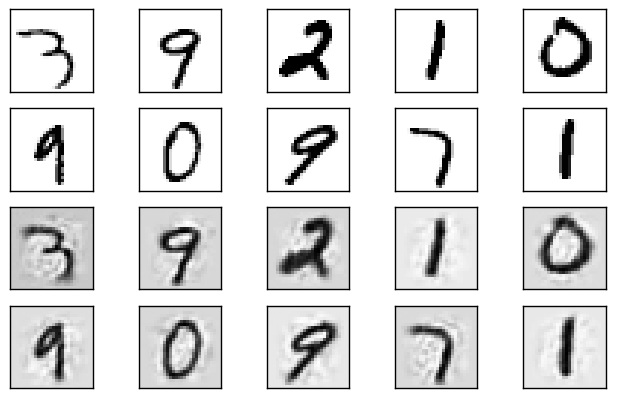
\includegraphics[scale=0.75]{AE-100-Test-Crop}
\end{figure}

\begin{figure}[]
\centering
\caption{Autoencoder results for 50 hidden layer neuron run}
\label{AE-50-figure}
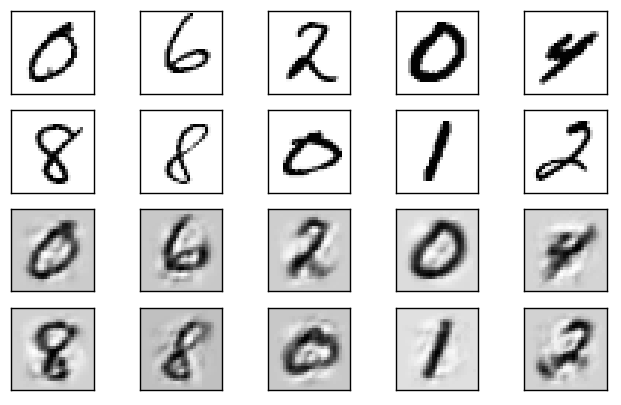
\includegraphics[scale=0.75]{AE-50-Test-Crop}
\end{figure}

\begin{figure}[]
\centering
\caption{Autoencoder results for 300 hidden layer neuron run}
\label{AE-300-figure}
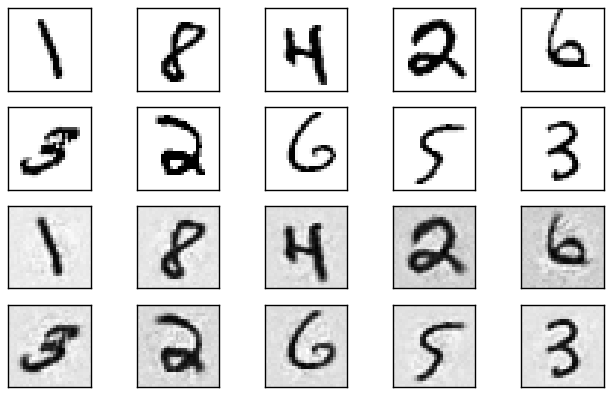
\includegraphics[scale=0.75]{AE-300-Test-Crop}
\end{figure}

\section{Discussion}
\label{sec:Discussion}

I found the results of this project quite interesting.  My initial expectation was that the feeforward classifier would be far outclassed by the autoencoder-augmented classifier, but that did not turn out to be the case.  Or at least, not with these settings on this data.  It may be that the MNIST data set simply does not require the model complexity that multiple layers allows.  It's also possible that the parameters I used were unfavourable to the autoencoder-augmented classifier, though I would be surprised if that were the case, as I tried many different configurations.  

The results show that at least for this application, the ANNs require a small learning rate.  In particular, the autoencoder completely falls apart moving from 0.01 to 0.1.  Moving to a smaller than 0.01 learning rate is also harmful, but to much lesser degree.  Learning rate seems like a difficult parameter to optimize.  I wonder if perhaps some of the sensitivity is due to the small ratio of training runs to the size of training set.  This ratio was 2:1 in all tests, meaning there is a high probability that some images are never evaluated during training.  

I found some of the results of the initial weight tests quite surprising.  I had heard that all zero initial weights interacted poorly with the backpropagation algorithm (which makes sense when you consider the math).  But I had no idea how much the size of the range for random weight initialization mattered.  Literature \cite{glorot2010understanding} suggested that when using tanh, the optimal range is $[-\sqrt{\frac{6}{fan_{in}+fan_{out}}}, \sqrt{\frac{6}{fan_{in}+fan_{out}}}]$, where $fan_{in}$ is the number of neurons in the preceding layer and $fan_{out}$ in the following layer.  Going from $[-1, 1]$ to the suggested range yielded over 30\% accuracy for the feeforward classifier, and 70\% for the autoencoder-augmented classifier! I would not have expected this to have such a strong impact. 

Varying the number of hidden layers seemed to have very little effect on the classification accuracy.  The autoencoder performed better at zero hidden layers.  This makes sense, of course, as with no hidden layers no real 'encoding' is required.  In a way, it shows by comparison that the performance of the autoencoder with default parameters is very good.  Adding a second hidden layer increased results by a tiny amount, and going up to three decreased them by a similarly small amount.  The conclusion seems to be that adding additional layers does little to help the classification.  

Interestingly, the classifier and autoencoder networks respond quite differently to changes in the size of the hidden layers.  The autoencoder improves steadily with increasing number of hidden layer neurons.  This seems like a sensible result to me; more neurons means more space to store information about the image.  On the other hand, the feedforward classifier had the best results at the smallest tested number of hidden layer neurons, 50.  My guess here is that more neurons in the hidden layer leads to overfitting.  I suspect the autoencoder does not have a problem with overfitting because it is trying to learn a much more general problem than the classifier.  

I would consider this project a success.  The feedforward classifier achieves a correct prediction rate of 94.66\% on the full 30000 image test set, which is a personal best for me on the MNIST dataset.  I was also impressed with the visual fidelity of the autoencoder, even at very low numbers of hidden layer neurons.  Unfortunately, the autoencoder-augmented classifier failed to impress.  I would be interested in trying it again, perhaps on a more complex image dataset.  

\pagebreak

\nocite{*}
\bibliographystyle{tktl}
\bibliography{reportbib}

\lastpage


\end{document}


